\documentclass{beamer}
\usetheme{default} 

\setbeamercolor{structure}{fg=green!40!black} 
\usebackgroundtemplate{
    \centering
\includegraphics[width=\paperwidth,height=\paperheight]{images/android_wall}
}
\setbeamertemplate{navigation symbols}{}

\usepackage[polish]{babel}
\usepackage[utf8x]{inputenc}
\usepackage{t1enc}
\usepackage{default}
\usepackage{listings}

\lstset{language=java, basicstyle=\small, commentstyle=\color{gray}}
\lstset{frame=single}

\usefoottemplate{
  \vbox{
    \tinycolouredline{structure!25}{
      \color{black}\textbf{	
        \insertshortauthor\hfill
        Android @ Szczecin 2011
      } 
    }
%    \tinycolouredline{structure}{
%      \color{white}\textbf{\insertshorttitle}\hfill
%    } 
  }
}

\title{Android @ Szczecin \\ 2011}
\author{Konrad Malawski \\ konrad.malawski@java.pl}

\begin{document}


\begin{frame}
 \begin{center}
  \Huge{AppWidgets}
 \end{center}
\end{frame}

\begin{frame}\frametitle{AppWidget}
\begin{itemize}
 \item Good news: Bardzo proste!
 \item AppWidget = specjalny BroadcastReciever
 \item a rozmiar etc, deklarujemy w \textbf{res/xml/my\_widget.xml}
\end{itemize}
\end{frame}


\begin{frame}[fragile]\frametitle{AppWidgetProvider}
\textbf{AppWidgetProvider}, musi zostać zarejestrowany w \textbf{AndroidManifest.xml} (w <application/>):
\begin{lstlisting}
<receiver android:name=".ui.appwidgets.MyWidgetProvider">
  <intent-filter>
    <action android:name="android.appwidget.action.APPWIDGET_UPDATE"/>
  </intent-filter>
  <meta-data android:name="android.appwidget.provider"
             android:resource="@xml/my_widget"/>
</receiver>
\end{lstlisting}
\end{frame}

\begin{frame}[fragile]\frametitle{res/xml/\textbf{my\_widget.xml}}
\begin{lstlisting}
<appwidget-provider xmlns:android="http://schemas.android.com/apk/res/android"
    android:minWidth="294dp"
    android:minHeight="72dp"
    android:updatePeriodMillis="86400000"
    android:previewImage="@drawable/preview_widget"
    android:initialLayout="@layout/widget">
</appwidget-provider>
\end{lstlisting}
Deklarowanie tego w XML jest wygodniejsze - mamy filtrowanie folderów (-v11).
\end{frame}



\begin{frame}[fragile]\frametitle{AppWidget - implementacja}
\begin{lstlisting}
public class MyWidgetProvider extends AppWidgetProvider {

  @Override
  public void onUpdate(Context context, 
                       AppWidgetManager appWidgetManager, 
                       int[] appWidgetIds) {

    // Provider obsluguje WIELE (N) widzetow!
    final int N = appWidgetIds.length;

    // aktualizujemy kazgego
    for (int i = 0; i < N; i++) {
      int appWidgetId = appWidgetIds[i];
      populateView(context, appWidgetManager, 
                            appWidgetId);
    }
  }
\end{lstlisting}
\end{frame}

\begin{frame}[fragile]\frametitle{AppWidget - implementacja}
\begin{lstlisting}
private void populateView(Context context, AppWidgetManager appWidgetManager, int appWidgetId) {
  // Przygotowujemy intent do odpalenia "on click"
  Intent intent = new Intent(context, ViewDetailsActivity.class);
  PendingIntent pendingIntent = PendingIntent.getActivity(context, 0, intent, 0);

  // rejestrujemy onClickListener'a troszke inaczej:
  RemoteViews views = new RemoteViews(context.getPackageName(), R.layout.widget);
  views.setOnClickPendingIntent(R.id.container, pendingIntent);
 
  // aktualizujemy widok widzetu (prosimy menagera o to)
  appWidgetManager.updateAppWidget(appWidgetId, views);
}
} // end of class
\end{lstlisting}
\end{frame}



\begin{frame}
\begin{center}
\Huge{Notifications}
\end{center}
\end{frame}

\begin{frame}\frametitle{Notificaion - przykład}
\begin{figure}
 \centering
 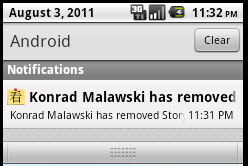
\includegraphics[width=0.7\textwidth]{images/notification_android_2_2}
\end{figure}
\end{frame}


\begin{frame}[fragile]\frametitle{NorificationManager}
\begin{lstlisting}
class MyActivity extends RoboActivity {
  
  @Inject
  NotificationManager notificationManager;

}
\end{lstlisting}
\pause Albo oczywiście \textbf{Service}.
\end{frame}


\begin{frame}[fragile]\frametitle{NorificationManager - 1/3}
\begin{lstlisting}
int icon = R.drawable.ic_kanbanery;
long when = System.currentTimeMillis();

Notification notification = new Notification(icon, title, when);

// ...
\end{lstlisting}
\end{frame}


\begin{frame}[fragile]\frametitle{NorificationManager - 2/3}
\begin{lstlisting}
int icon = R.drawable.ic_kanbanery;
long when = System.currentTimeMillis();

Notification notification = new Notification(icon, title, when);

Intent notificationIntent = new Intent(this, ColumnsActivity.class);
PendingIntent onClickIntent = PendingIntent.getActivity(this, 0, notificationIntent, 0);

// ...
\end{lstlisting}
\end{frame}

\begin{frame}[fragile]\frametitle{NotificationManager - 3/3}
\begin{lstlisting}
int icon = R.drawable.ic_kanbanery;
long when = System.currentTimeMillis();

Notification notification = 
                 new Notification(icon, title, when);

Intent notificationIntent = new Intent(this, 
                              ColumnsActivity.class);
PendingIntent contentIntent = PendingIntent
        .getActivity(this, 0, notificationIntent, 0);

notification.setLatestEventInfo(context, title, 
                                msg, contentIntent);
notification.flags = Notification.FLAG_AUTO_CANCEL;


notificationManager.notify(ACTION_ID, // explain 
                           notification);
\end{lstlisting}
\end{frame}






\end{document}
